% last updated in April 2002 by Antje Endemann
% Based on CVPR 07 and LNCS, with modifications by DAF, AZ and elle, 2008 and AA, 2010
% Modified for DAGM 2010 by SR
% Modified for DAGM 2011 by HF&CB, updated lncs.cls and splncs03.bst
% Modified for DAGM-OAGM 2012 by TP, updated lncs.cls and splncs03.bst
% Modified for GCPR 2013 by MH
% Modified for GCPR 2014 by XJ
% Modified for GCPR 2015 by JG, updated lncs.cls and splncs03.bst

\documentclass[runningheads]{llncs}

\usepackage{makeidx}
\usepackage{graphicx}
\usepackage{amsmath,amssymb} % define this before the line numbering.
\usepackage{color}
\usepackage{paralist}

\renewcommand{\ttdefault}{pcr}
%\lstloadlanguages{Pascal}
%\lstset{
%	language=Pascal,
%	captionpos=t,
%	tabsize=2,
%	breakatwhitespace=true,
%	showspaces=false,
%	showstringspaces=false,
%}


% Definition of \DAGMreviewversion which
% defines the use of line numbers etc.
\newcommand\DAGMreviewversion{
	\usepackage{lineno}
	\usepackage{color}
	\renewcommand\thelinenumber{\color[rgb]{0.2,0.5,0.8}\normalfont\sffamily\scriptsize\arabic{linenumber}\color[rgb]{0,0,0}}
	\renewcommand\makeLineNumber {\hss\thelinenumber\ \hspace{6mm} \rlap{\hskip\textwidth\ \hspace{6.5mm}\thelinenumber}} 
	\linenumbers
}

% Please activate this command (\DAGMreviewversion) for a draft
% version of your manuscript which will be used during the review
% process.
% DO NOT USE this command for the camera ready version of your paper.
\DAGMreviewversion

\usepackage{xspace} % context sensitive space after macros
\makeatletter
\DeclareRobustCommand\onedot{\futurelet\@let@token\@onedot}
\def\@onedot{\ifx\@let@token.\else.\null\fi\xspace}
\def\eg{{e.g}\onedot} \def\Eg{{E.g}\onedot}
\def\ie{{i.e}\onedot} \def\Ie{{I.e}\onedot}
\def\cf{{c.f}\onedot} \def\Cf{{C.f}\onedot}
\def\etc{{etc}\onedot} \def\vs{{vs}\onedot}
\def\wrt{w.r.t\onedot} \def\dof{d.o.f\onedot}
\def\etal{{et al}\onedot}

\usepackage{tabularx}
\newcolumntype{Y}{>{\centering\arraybackslash}X}

\usepackage[tight]{subfigure}
\usepackage{tikz}
\usetikzlibrary{calc}
\usetikzlibrary{matrix}
\usetikzlibrary{arrows}
\usetikzlibrary{calc}
\usetikzlibrary{decorations.pathreplacing} % braces for tikz
\usetikzlibrary{positioning,shapes.geometric}
\usetikzlibrary{backgrounds}
\usepackage{mathtools}
\usepackage{pgfplots}
\usepackage{pgfplotstable}
\usepackage{multirow}
\usepackage{xcolor}

% using equal sign in column labels
\newcommand{\pgfequalsign}{=}
\newcommand\refbsdnyu[1]{% positions two related legendimages in one cell
  \raisebox{1.5pt}{\ref{plot:#1bsd}}\llap{\raisebox{-1pt}{\ref{plot:#1nyu}}}%
}

% TODO: FH black?
\pgfplotscreateplotcyclelist{comparison bsd}{%
	teal,mark=star,solid\\% NC
	orange,mark=star,solid\\% FH
	red,mark=star,solid\\% QS
	green!40!black,mark=star,solid\\% TP
	blue,mark=star,solid\\% SLIC
	%black,mark=star,solid\\% SLIC3D
	violet,mark=star,solid\\% CIS
	cyan,mark=star,solid\\% ERS
	brown,mark=star,solid\\% PB
	teal,mark=star,dashed\\% SEEDS
	orange,mark=star,dashed\\% reSEEDS
	%red,mark=star,dashed\\% reSEEDS3Dn
	%blue,mark=star,dashed\\% DASP
	green!40!black,mark=star,dashed\\% TPS
	violet,mark=star,dashed\\% CRS
	%brown,mark=star,dashed\\% VCCS
}
\pgfplotscreateplotcyclelist{comparison nyu}{%
	teal,mark=star,solid\\% NC
	orange,mark=star,solid\\% FH
	red,mark=star,solid\\% QS
	green!40!black,mark=star,solid\\% TP
	blue,mark=star,solid\\% SLIC
	%black,mark=star,solid\\% SLIC3D
	violet,mark=star,solid\\% CIS
	cyan,mark=star,solid\\% ERS
	brown,mark=star,solid\\% PB
	teal,mark=star,dashed\\% SEEDS
	orange,mark=star,dashed\\% reSEEDS
	red,mark=star,dashed\\% reSEEDS3Dn
	blue,mark=star,dashed\\% DASP
	green!40!black,mark=star,dashed\\% TPS
	violet,mark=star,dashed\\% CRS
	brown,mark=star,dashed\\% VCCS
}
\pgfplotscreateplotcyclelist{runtime nyu}{%
	%teal,mark=star,solid\\% NC
	orange,mark=star,solid\\% FH
	%red,mark=star,solid\\% QS
	%green!40!black,mark=star,solid\\% TP
	blue,mark=star,dotted\\% SLIC 1it
	blue,mark=star,solid\\% SLIC
	%black,mark=star,solid\\% SLIC3D
	%violet,mark=star,solid\\% CIS
	%cyan,mark=star,solid\\% ERS
	%brown,mark=star,solid\\% PB
	teal,mark=star,dotted\\% SEEDS 1it
	teal,mark=star,dashed\\% SEEDS
	orange,mark=star,dotted\\% reSEEDS 1it
	orange,mark=star,dashed\\% reSEEDS
	red,mark=star,dashed\\% reSEEDS3Dn
	blue,mark=star,dashed\\% DASP
	%green!40!black,mark=star,dashed\\% TPS
	%violet,mark=star,dashed\\% CRS
	brown,mark=star,dashed\\% VCCS
}

\newcommand{\plotfontsize}{\scriptsize}
\pgfplotsset{every axis/.append style={tick label style={/pgf/number format/fixed},font=\plotfontsize,ylabel near ticks,xlabel near ticks,grid=major}}
\pgfplotstableset{%
    highlightrow/.style={%
        postproc cell content/.append code={%
           \count0=\pgfplotstablerow
            \advance\count0 by1
            \ifnum\count0=#1
            %\pgfkeysalso{@cell content/.add={$\bf}{$}}
            \pgfkeysalso{@cell content=\textit{##1}}%
            \fi
        },
    },
}
\pgfplotstableset{%
  cignore row/.style={
    row predicate/.append code={
      \ifnum#1=\pgfplotstablerow\relax
        \pgfplotstableuserowfalse
      \fi
    }
  },
}

% http://tex.stackexchange.com/questions/30720/footnote-without-a-marker
\newcommand\blfootnote[1]{%
  \begingroup
  \renewcommand\thefootnote{}\footnote{#1}%
  \addtocounter{footnote}{-1}%
  \endgroup
}

% http://tex.stackexchange.com/questions/42619/x-mark-to-match-checkmark
\usepackage{pifont}% http://ctan.org/pkg/pifont
\newcommand{\cmark}{\ding{51}}%
\newcommand{\xmark}{\ding{55}}%

% http://tex.stackexchange.com/questions/31672/column-and-row-padding-in-tables
\def\arraystretch{1.5}
\setlength\tabcolsep{0.75mm}

\begin{document}
	\pagestyle{headings}
	\mainmatter

	% Insert your submission number here
	\def\GCPR15SubNumber{78}

	% Replace with your title
	\title{Superpixel Segmentation: An Evaluation}

	% DO NOT MODIFY these for the draft version that is used for the
	% review process.
	\titlerunning{GCPR 2015 Submission \#\GCPR15SubNumber{}. CONFIDENTIAL REVIEW COPY.}
	\authorrunning{GCPR 2015 Submission \#\GCPR15SubNumber{}. CONFIDENTIAL REVIEW COPY.}
	\author{David Stutz}
	\institute{Computer Vision Group, RWTH Aachen University (Paper ID \GCPR15SubNumber)}

	\maketitle
	%\vspace{-2mm}
	
	\begin{abstract}
		In recent years, superpixel algorithms have become a standard tool in computer vision and many approaches have been proposed. However, different evaluation methodologies make direct comparison difficult. We address this shortcoming with a thorough and fair comparison of thirteen state-of-the-art superpixel algorithms. To include algorithms utilizing depth information we present results on both the Berkeley Segmentation Dataset \cite{ArbelaezMaireFowlkesMalik:2011} and the NYU Depth Dataset \cite{SilbermanHoiemKohliFergus:2012}. Based on qualitative and quantitative aspects, our work allows to guide algorithm selection by identifying important quality characteristics.\blfootnote{Recommended for submission to YRF2015 by Prof. Dr. Bastian Leibe.}
	\end{abstract}
    %\vspace{-2mm}
    
    \vspace{-1mm}
	\section{Introduction}
	\vspace{-0.5mm}
	
	The term superpixel was introduced by Ren and Malik in 2003 \cite{RenMalik:2003} and is used to describe a group of pixels similar in color or other low-level properties. The concept of superpixels is motivated by two important aspects \cite{RenMalik:2003}: firstly, pixels do not represent natural entities but are merely a result of discretization; and secondly, the high number of pixels in large images prevents many algorithms from being computationally feasible.
	% At this point, Ren and Malik introduce superpixels as more natural entities -- grouping pixels which perceptually belong together.

    Superpixels have actively been used for a wide range of applications such as classical segmentation \cite{RenMalik:2003,RohkohlEngel:2007}, semantic segmentation \cite{GuptaArbelaezMalik:2013}, stereo matching \cite{YuhangZhangHartleyMashfordBurn:2011} or tracking \cite{ShuWangHuchuanLuFanYangMingHsuanYang:2011} and numerous superpixel algorithms have been proposed.
    % Usually, authors agree on requirements such as connectivity \cite{LevinshteinStereKutulakosFleetDickinsonSiddiqi:2009}, boundary adherence \cite{LevinshteinStereKutulakosFleetDickinsonSiddiqi:2009,AchantaShajiSmithLucchiFuaSuesstrunk:2010,LiuTuzelRamalingamChellappa:2011} and compactness \cite{LevinshteinStereKutulakosFleetDickinsonSiddiqi:2009,SchickFischerStiefelhagen:2012}.
% \begin{inparaenum}[(i)]
% 	\item superpixels should respect object boundaries;
% 	\item superpixels should be generated as efficiently as possible;
% 	\item and superpixels should not lower the achievable performance of subsequent processing steps.
% \end{inparaenum}
% Additional requirements may include compactness \cite{LevinshteinStereKutulakosFleetDickinsonSiddiqi:2009,SchickFischerStiefelhagen:2012} and connectivity \cite{LevinshteinStereKutulakosFleetDickinsonSiddiqi:2009}.
    However, keeping an overview of the different approaches and their suitability for specific applications is difficult. This is caused by varying experimental setups and metrics used for evaluation \cite{NeubertProtzel:2012}. Furthermore, only few publications are devoted to a thorough comparison of existing algorithms.
    
    In this paper, we address this shortcoming and present an extensive comparison of thirteen state-of-the-art superpixel algorithms. In Section \ref{sec:related-work} we discuss important related work regarding the comparison of superpixel algorithms and subsequently we survey existing superpixel algorithms. In Section \ref{sec:datasets} we discuss relevant datasets and introduce our benchmark in Section \ref{sec:benchmark}. Finally, in Section \ref{sec:evaluation}, we present a qualitative and quantitative comparison of the superpixel algorithms, before concluding in Section \ref{sec:conclusion}.
    
    \vspace{-1mm}
    \section{Related Work}
    \vspace{-0.5mm}
    \label{sec:related-work}
    
    %\vspace{-1mm}
    %\subsection{Comparison and Evaluation}
    %\vspace{-0.5mm}
    
    There are only few publications devoted to the comparison of existing superpixel algorithms in a consistent framework: to the best of our knowledge these are \cite{SchickFischerStiefelhagen:2012}, \cite{AchantaShajiSmithLucchiFuaSuesstrunk:2012} and \cite{NeubertProtzel:2012}. However, these publications cannot include several recent algorithms (for example \cite{VanDenBerghBoixRoigCapitaniVanGool:2012,PaponAbramovSchoelerWoergoetter:2013,WeikersdorferGossowBeetz:2012}). Meanwhile, authors tend to include a brief evaluation intended to show superiority of their proposed superpixel algorithm over selected existing approaches (for example \cite{LiuTuzelRamalingamChellappa:2011,VekslerBoykovMehrani:2010,VanDenBerghBoixRoigCapitaniVanGool:2012,VanDenBerghBoixRoigCapitaniVanGool:2012,WeikersdorferGossowBeetz:2012,PaponAbramovSchoelerWoergoetter:2013}).
    However, these results are not comparable across publications.
    
    % When considering depth information for superpixel segmentation, we distinguish supervoxel algorithms\footnote{Note the difference to supervoxel algorithms where the third dimension is given as the temporal domain of a video, see \cite{XuCorso:2012}.}, operating directly within a point cloud and superpixel algorithms utilizing depth as additional feature dimension. One of the former is Voxel-Cloud Connectivity Segmentation (\textit{VCCS}) \cite{PaponAbramovSchoelerWoergoetter:2013} performing $K$-means clustering in a $26$-adjacency graph constructed from a voxelized point cloud. Weikersdorfer \etal \cite{WeikersdorferGossowBeetz:2012} propose Depth-Adaptive Superpixels (\textit{DASP}), an algorithm of the latter kind, performing $K$-means clustering in color and $(x,y,z)$-coordinate space built by projecting pixels back into a world coordinate system.
    
    %\vspace{-1mm}
    %\section{Survey}
    %\vspace{-0.5mm}
    %\label{sec:survey}
    
    \vspace{-1mm}
    \subsection{Superpixel Algorithms}
    \vspace{-0.5mm}
    \label{sec:survey}
    
    \begin{table}[t]
        \caption{Overview of all evaluated superpixel algorithms ordered by year of publication. In Row 3, we categorize the algorithms in either graph-based approaches (gb) or gradient ascent approaches (ga) \cite{AchantaShajiSmithLucchiFuaSuesstrunk:2012}. Furthermore, in Row 4, we note the programming language of the evaluated implementations as it may influence the runtime reported in Section \ref{subsec:quantitative} (M refers to MatLab). We distinguish algorithms offering direct control over the number of superpixels (Row 5), algorithms providing a compactness parameter (Row 6) and algorithms using depth information (Row 7).}
        \label{table:survey}
        \centering
        {\scriptsize
        \begin{tabular}{| l | c | c | c | c | c | c | c | c | c | c | c | c | c |}
        \hline
            & \textit{NC} & \textit{FH} & \textit{QS} & \textit{TP} & \textit{SLIC} & \textit{CIS} & \textit{ERS} & \textit{PB} & \textit{CRS} & \textit{SEEDS} & \textit{TPS} & \textit{DASP} & \textit{VCCS}\\\hline\hline
            Ref. & \cite{RenMalik:2003} & \cite{FelzenswalbHuttenlocher:2004} & \cite{VedaldiSoatto:2008} & \cite{LevinshteinStereKutulakosFleetDickinsonSiddiqi:2009} & \cite{AchantaShajiSmithLucchiFuaSuesstrunk:2010} & \cite{VekslerBoykovMehrani:2010} & \cite{LiuTuzelRamalingamChellappa:2011} & \cite{ZhangHartleyMashfordBurn:2011} & \cite{MesterConradGuevara:2011} & \cite{VanDenBerghBoixRoigCapitaniVanGool:2012} & \cite{DaiTangHuazhaFuXiaochunCao:2012} & \cite{WeikersdorferGossowBeetz:2012} & \cite{PaponAbramovSchoelerWoergoetter:2013}\\
            Year & 2003 & 2004 & 2008 & 2009 & 2010 & 2010 & 2011 & 2011 & 2011 & 2012 & 2012 & 2012 & 2013\\
            Cat. & gb & gb & ga & ga & ga & gb & gb & gb & ga & ga & gb & ga & ga\\
            Impl. & C/M & C++ & C/M & C/M & C++ & C++ & C++ & C++ & C++ & C++ & C/M & C++ & C++\\
            Sup. & \cmark & \xmark & \xmark & \cmark & \cmark & \cmark & \cmark & \cmark & \cmark & \cmark & \cmark & \cmark & \xmark\\
            Comp. & \xmark & \xmark & \xmark & \xmark & \cmark & \xmark & \xmark & \xmark & \cmark & \xmark & \xmark & \cmark & \cmark\\
            Depth & \xmark & \xmark & \xmark & \xmark & \xmark & \xmark & \xmark & \xmark & \xmark & \xmark & \xmark & \cmark & \cmark\\\hline
        \end{tabular}
        }
    \end{table}
    
    Table \ref{table:survey} gives an overview of all evaluated superpixel algorithms. We categorize the algorithms according to criteria we find important for evaluation and algorithm selection. Roughly, the algorithms can be categorized as either graph-based approaches or gradient ascent approaches \cite{AchantaShajiSmithLucchiFuaSuesstrunk:2012}. Furthermore, we distinguish algorithms offering direct control over the number of superpixels as well as algorithms providing a compactness parameter. Overall, we evaluated thirteen state-of-the-art superpixel algorithms including three algorithms utilizing depth information.
    We also note that there are additional superpixel algorithms \cite{RohkohlEngel:2007,MoorePrinceWarrellMohammedJones:2008,DruckerMacCormick:2009,ZengWangWangGanZha:2011,PerbetStengerMaki:2012,SivaWong:2014} for which evaluation was not possible due to the lack of open source code.
    
    %% This Section is intended to give a brief survey of existing superpixel algorithms focussing on algorithms evaluated in Section \ref{sec:evaluation}. 
    % Ren and Malik \cite{RenMalik:2003} originally used the Normalized Cuts (\textit{NC}, 2003) algorithm \cite{ShiMalik:2000} to generate superpixels.
    % Similarly, the graph-based image segmentation algorithm by Felzenswalb and Huttenlocher (\textit{FH}, 2004) \cite{FelzenswalbHuttenlocher:2004} as well as the mode-seeking algorithm Quick Shift (\textit{QS}, 2008) \cite{VedaldiSoatto:2008} are commonly used for superpixel segmentation.
    %% In 2004, Felzenswalb and Huttenlocher \cite{FelzenswalbHuttenlocher:2004} proposed a graph-based approach to image segmentation, referred to as \textit{FH}, which is commonly used as superpixel algorithm.
    %% Proposed several years later, Rohkohl and Engel \cite{RohkohlEngel:2007} refine an initial superpixels segmentation -- a hexagonal grid -- by exchanging boundary pixels based on color similarity which we refer to as Superpixels using Pairwise Pixel Similarities (\textit{SPPS}).
    %% Similarly, Vedaldi and Soatto \cite{VedaldiSoatto:2008} proposed Quick Shift (\textit{QS}) representing a mode-seeking algorithm that may be used to generate superpixels.
    %% Also proposed in 2008, Superpixel Lattices (\textit{SL}) \cite{MoorePrinceWarrellMohammedJones:2008} attempts to create a regular grid of superpixels in order to maintain several desirable properties available within the pixel grid.
    % Following these early approaches, Levinshtein \etal \cite{LevinshteinStereKutulakosFleetDickinsonSiddiqi:2009} introduced TurboPixels (\textit{TP}, 2009), representing superpixels as an evolving contour driven by image content and compactness constraints.
    % In contrast, Simple Linear Iterative Clustering (\textit{SLIC}, 2010) \cite{AchantaShajiSmithLucchiFuaSuesstrunk:2010} is based on local $K$-means clustering and quickly became a popular superpixel algorithm.
    % \textit{SLIC} was followed by several graph-based approaches, such as Constant Intensity Superpixels (\textit{CIS}, 2010) \cite{VekslerBoykovMehrani:2010}, Entropy Rate Superpixels (\textit{ERS}, 2011) \cite{LiuTuzelRamalingamChellappa:2011} and Pseudo-Boolean Superpixels (\textit{PB}, 2011) \cite{ZhangHartleyMashfordBurn:2011}. While \textit{ERS} greedily optimizes an objective function based on the entropy rate of random walks, \textit{CIS} and \textit{PB} use classical methods to assign labels to individual pixels: $\alpha$-expansion \cite{BoykovVekslerZabih:2001} and max-flow, respectively.
    % Mester \etal \cite{MesterConradGuevara:2011} proposed a statistical approach to superpixel segmentation called Contour-Relaxed Superpixels (\textit{CRS}, 2011).
    % Motivated by the high runtime of many approaches, Van den Bergh \etal \cite{VanDenBerghBoixRoigCapitaniVanGool:2012} proposed Superpixels Extracted via Energy-Driven Sampling (\textit{SEEDS}, 2012) aimed for real-time applications by optimizing an objective function using hill-climbing.
    %% In the same year, Constant Intensity Superpixels (\textit{CIS}), proposed by Veksler \etal \cite{VekslerBoykovMehrani:2010}, use $\alpha$-expansion \cite{BoykovVekslerZabih:2001} to assign pixels to initially overlapping squares.
    %% In 2011, Entropy Rate Superpixels (\textit{ERS}) \cite{LiuTuzelRamalingamChellappa:2011}, Pseudo-Boolean Superpixels (\textit{PB}) \cite{ZhangHartleyMashfordBurn:2011} and Contour-Relaxed Superpixels (\textit{CRS}) \cite{ConradMertzMester:2013} were introduced. While \textit{ERS} is a graph-based approach greedily optimizing an energy based on the entropy rate of random walks, \textit{PB} covers the image with overlapping horizontal and vertical strips and assigns pixels to these strips using max-flow. In contrast to the algorithms introduced so far, \textit{CRS} represents a statistical approach, assuming that each superpixel is a stochastic process generating the underlying image.
    %% Further, Structure Sensitive Superpixels (\textit{SSS}) \cite{ZengWangWangGanZha:2011} was proposed, an algorithm based on Lloyd's algorithms and a custom geodesic distance, and Perbet \etal proposed Homogeneous Superpixels (\textit{HS}) \cite{PerbetStengerMaki:2012}, a graph-based approach utilizing Markov Clustering.
    %% In 2012, van den Bergh \etal \cite{VanDenBerghBoixRoigCapitaniVanGool:2012} proposed \textit{SEEDS}, Superpixels Extracted via Energy-Driven Sampling, which exchanges blocks of pixels or individual pixels between neighboring superpixels based on color similarity.
    % TODO: Better transition!
    % Topology Preserved Superpixels (\textit{TPS}, 2012) \cite{DaiTangHuazhaFuXiaochunCao:2012} generates a regular grid of superpixels by connecting initial seed points based on edge information.
    % Recently, Weikersdorfer \etal \cite{WeikersdorferGossowBeetz:2012} proposed Depth-Adaptive Superpixels (\textit{DASP}, 2012) similar to \textit{SLIC} but utilizing depth information.
    % In contrast, Papon \etal \cite{PaponAbramovSchoelerWoergoetter:2013} proposed Voxel-Cloud-Connectivity Segmentation (\textit{VCCS}, 2013) directly operating on point clouds.
    % We also note that there are additional superpixel algorithms \cite{RohkohlEngel:2007,MoorePrinceWarrellMohammedJones:2008,DruckerMacCormick:2009,ZengWangWangGanZha:2011,PerbetStengerMaki:2012,SivaWong:2014} for which evaluation was not possible due to the lack of open source code.
    
    \vspace{-1mm}
    \section{Datasets}
    \vspace{-0.5mm}
    \label{sec:datasets}
    
    % TODO: describe evaluation methodology!
    As popular dataset for image segmentation and contour detection, the Berkeley Segmentation Dataset \cite{ArbelaezMaireFowlkesMalik:2011}, referred to as BSDS500, consists of $500$ natural images of size $482 \times 321$ ($200$ training images, $100$ validation images, $200$ test images). The provided ground truth segmentations, at least five per image, have been obtained from different persons and reflect the difficult nature of image segmentation.
    % This also results in a fair evaluation as, for each superpixel segmentation and given a particular metric, we can choose the best ground truth segmentation for evaluation.
    % In Section \ref{sec:evaluation}, per image, we take the best ground truth segmentation instead of averaging 
    % In practice, concerning all measures based on ground truth segmentations presented in this chapter, for each image we choose the ground truth segmentation resulting in the best value and subsequently average over all images. However, note that some of the measures provided as part of the Berkeley Segmentation Benchmark offer natural extensions to multiple ground truth segmentations, as for example the Probabilistic Rand Index \cite{UnnikrishnanPantofaruHebert:2007}, see appendix \ref{chapter:appendix-berkeley-segmentation-benchmark}.
    
    % The first version of the NYU Depth Dataset, in the following referred to as NYUV1, was introduced in \cite{SilbermanFergus:2011} by Silberman \etal. The dataset comprises $2284$\footnote{Although, Silberman \etal mention $2347$ labeled frames \cite{SilbermanFergus:2011}, we found that, actually, the dataset comprises only $2284$ labeled frames.} labeled frames taken from video sequences showing six different indoor scenes. The video sequences were taken by a calibrated Microsoft Kinect \cite{SilbermanFergus:2011} such that depth information is accessible. The frames were annotated using the LabelMe tool \cite{RussellTorralbaMurphyFreeman:2008} resulting in around $1000$ classes which are highly redundant \cite{SilbermanFergus:2011}.

    In contrast to the natural images of the BSDS500, The NYU Depth Dataset \cite{SilbermanHoiemKohliFergus:2012}, referred to as NYUV2, comprises $1449$ images of different indoor scenes (we chose $200$ validation images and $400$ test images including most of the scenes). For all images, pre-processed depth images are provided. As these images have been undistorted and aligned with the color images, we crop the original images of size $640 \times 480$ to $608 \times 448$ pixels. In addition, following Ren and Bo \cite{RenBo:2012},
    % although Silberman \etal state that the annotators were instructed to provide a dense labeling,
    we remove small unlabeled regions and combine class and instance labels to guarantee connected ground truth segments. Overall, difficult lighting conditions and cluttered scenes contribute to the difficulty of the NYUV2.
    % TODO: clear label and instance merging!
    
    % The second version of the NYU Depth Dataset \cite{SilbermanHoiemKohliFergus:2012}, NYUV2, adds further variety in the form of indoor scenes from different cities as well as commercial accommodations. The dataset comprises $1449$ labeled frames with a total of $894$ classes \cite{SilbermanHoiemKohliFergus:2012}. Every instance of a particular class within a single frame gets a unique instance label. Following Ren and Bo \cite{RenBo:2012} we combine class labels and instance labels to generate ground truth segmentations compatible with the Berkeley Segmentation Benchmark. Although Silberman \etal state that the annotators were instructed to provide a dense labeling of the scenes, the images often contain small unlabeled regions in between larger labeled regions, see Figure~\ref{fig:datasets-nyu-depth-dataset-labels}. Therefore, based on code provided by Ren and Bo \cite{RenBo:2012}, we remove these small background regions. Furthermore, bad lighting as well as cluttered scenes account for the difficulty of the NYUV2. However, this also represents an appropriate contrast to the natural images of the BSDS500.
    
    \vspace{-1mm}
    \section{Benchmark}
    \vspace{-0.5mm}
    \label{sec:benchmark}
    
    We use an extended version of the Berkeley Segmentation Benchmark, introduced by Arbel\'aez \etal \cite{ArbelaezMaireFowlkesMalik:2011}, to evaluate superpixel algorithms. Among other metrics, the benchmark includes Boundary Recall ($Rec$) and Undersegmentation Error ($UE$) \cite{LevinshteinStereKutulakosFleetDickinsonSiddiqi:2009,NeubertProtzel:2012} as primary metrics to assess superpixel algorithms. 
    %Here, we focus on the most commonly used metrics, namely Boundary Recall and Undersegmentation Error, and exclude the remaining metrics for brevity.
    % Further, several metrics provided by the Berkeley Segmentation Dataset are not suitable for evaluating superpixel algorithms, as for example Boundary Precision or Segmentation Covering.
    
    Boundary Recall is part of the Precision-Recall Framework \cite{MartinFowlkesMalik:2004} originally used to evaluate contour detectors. Treating region boundaries of a superpixel segmentation as contours, Boundary Recall represents the fraction of boundary pixels correctly detected by the superpixel algorithm. As superpixels are expected to adhere to boundaries, high Boundary Recall is desirable.
    
    Undersegmentation Error, as originally proposed by Levinshtein \etal \cite{LevinshteinStereKutulakosFleetDickinsonSiddiqi:2009}, measures the ``bleeding'' of superpixels with respect to a ground truth segmentation.
    % However, the original definition as used in \cite{LevinshteinStereKutulakosFleetDickinsonSiddiqi:2009}, \cite{LiuTuzelRamalingamChellappa:2011} and \cite{VekslerBoykovMehrani:2010} has several disadvantages including its difficult interpretability and comparability as the it is not constrained to lie in $[0,1]$ \cite{AchantaShajiSmithLucchiFuaSuesstrunk:2012,NeubertProtzel:2012}.
    We implemented the corrected formulation proposed by Neubert and Protzel \cite{NeubertProtzel:2012} computing an error in the range of $[0,1]$. Low Undersegmentation Error is preferable as each superpixel is expected to cover at most one ground truth segment.
    % TODO: is expected to cover -> optimally only covers
    
    \vspace{-1mm}
    \section{Evaluation and Comparison}
    \vspace{-0.5mm}
    \label{sec:evaluation}
    
    % In addition to the superpixel algorithms introduced in Section \ref{sec:survey}, our comparison includes a re-implementation of \textit{SEEDS}, closely following \cite{VanDenBerghBoixRoigCapitaniVanGool:2012} and referred to as \textit{reSEEDS}, and an extension of \textit{reSEEDS} to depth information, referred to as \textit{reSEEDS3D}. Further details on \textit{reSEEDS} and \textit{reSEEDS3D}, all other evaluated algorithms and their parameters as well as additional experiments can be found in \cite{Stutz:2014}.
    In addition to the superpixel algorithms introduced in Section \ref{sec:survey}, we include a 2D and 3D re-implementation of \textit{SEEDS}, called \textit{reSEEDS} and \textit{reSEEDS3D}, respectively. Further details can be found in \cite{Stutz:2014}.
    
    Our comparison is split into a qualitative part, examining the visual quality of the generated superpixels, and a quantitative part based on Boundary Recall, Undersegmentation Error and runtime.
    To ensure a fair comparison, the parameters have been chosen to jointly optimize Boundary Recall and Undersegmentation Error using discrete grid search.
    % Where possible, grid search was guided by parameter values reported in the literature
    % Where possible, grid search was guided by default parameters reported in the literature.
    Parameter optimization was performed on the validation sets while comparison is performed on the test sets.
    
    % Further experiments as well as details on all evaluated algorithms and the corresponding parameters can be found in \cite{Stutz:2014}.
    
    \vspace{-1.5mm}
    \subsection{Qualitative}
    \vspace{-0.5mm}
    \label{subsec:qualitative}

    The visual appearance of superpixels is determined by compactness and regularity
    -- properties that may also have strong influence on possible applications.
    % as compact and regular superpixels may be preferrable for specific applications.
    % , that is compact and regular superpixels are perceived as visual appealing.
    % Here, compactness refers to the shape of superpixels, while regularity refers to positioning and size.
    Figures \ref{fig:qualitative-bsd} and \ref{fig:qualitative-nyu} present results on the BSDS500 and NYUV2, respectively, obtained after parameter optimization.
    % On the NYUV2, depth information was used for \textit{reSEEDS3D}, \textit{DASP} and \textit{VCCS}.
    % Note that these results are merely a weak indicator for performance on similar images.
    We note that these images are intended to be as representative as possible, however, generated superpixel segmentations may vary across different images.
    
    \begin{figure}[t]
        \begin{tabularx}{\linewidth}{@{}Y@{}Y@{}Y@{}Y@{}Y@{}Y@{}Y@{}}
            \resizebox{0.99\linewidth}{!}{
                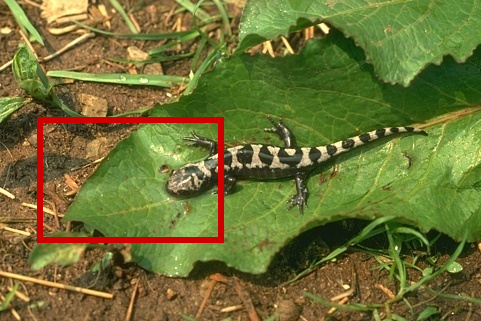
\includegraphics{pictures/bsd-test-2}
            }
            &
            %\resizebox{\linewidth}{!}{
            %    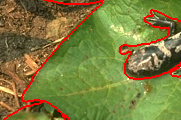
\includegraphics{pictures/bsd-test-2-contours-excerpt}
            %}
            %&
            \resizebox{\linewidth}{!}{
                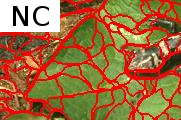
\includegraphics{pictures/bsd-test-2-nc-excerpt}
            }
            &
            \resizebox{\linewidth}{!}{
                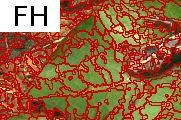
\includegraphics{pictures/bsd-test-2-fh-excerpt}
            }
            &
            \resizebox{\linewidth}{!}{
                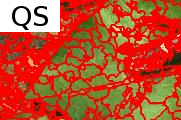
\includegraphics{pictures/bsd-test-2-qs-excerpt}
            }
            &
            \resizebox{\linewidth}{!}{
                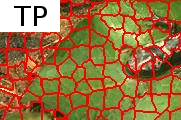
\includegraphics{pictures/bsd-test-2-tp-excerpt}
            }
            &
            \resizebox{\linewidth}{!}{
                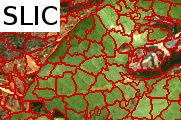
\includegraphics{pictures/bsd-test-2-orislic-excerpt}
            }
            &
            \resizebox{\linewidth}{!}{
                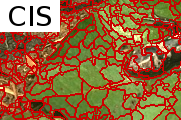
\includegraphics{pictures/bsd-test-2-cis-excerpt}
            }
            \\
            &
            \resizebox{\linewidth}{!}{
                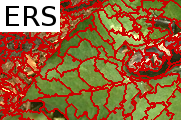
\includegraphics{pictures/bsd-test-2-ers-excerpt}
            }
            &
            \resizebox{\linewidth}{!}{
                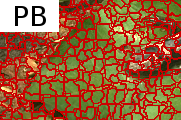
\includegraphics{pictures/bsd-test-2-pb-excerpt}
            }
            &
            \resizebox{\linewidth}{!}{
                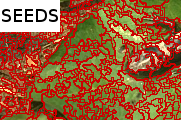
\includegraphics{pictures/bsd-test-2-oriseedsmp-excerpt}
            }
            &
            \resizebox{\linewidth}{!}{
                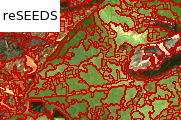
\includegraphics{pictures/bsd-test-2-reseedsmp-excerpt}
            }
            &
            \resizebox{\linewidth}{!}{
                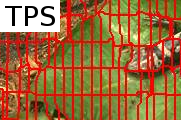
\includegraphics{pictures/bsd-test-2-tps-excerpt}
            }
            &
            \resizebox{\linewidth}{!}{
                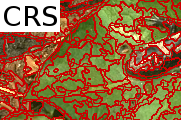
\includegraphics{pictures/bsd-test-2-crs-excerpt}
            }
        \end{tabularx}
        \vspace{-2.5mm}
        \caption{Superpixel segmentations obtained for an example image from the BSDS500. From left to right, top to bottom: original image, \textit{NC}, \textit{FH}, \textit{QS}, \textit{TP}, \textit{SLIC}, \textit{CIS}, \textit{ERS}, \textit{PB}, \textit{SEEDS}, \textit{reSEEDS}, \textit{TPS} and \textit{CRS}. Approximately $600$ superpixels have been generated for the whole image.}
        \label{fig:qualitative-bsd}
    \end{figure}
    
    \begin{figure}[b]
        \begin{tabularx}{\linewidth}{@{}Y@{}Y@{}Y@{}Y@{}Y@{}Y@{}Y@{}Y@{}}
            \resizebox{0.99\linewidth}{!}{
                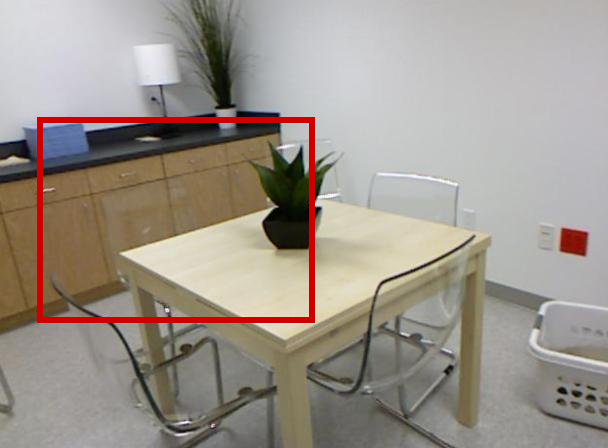
\includegraphics{pictures/nyu-test-1}
            }
            &
            %\resizebox{\linewidth}{!}{
            %    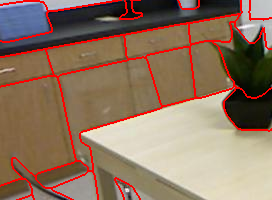
\includegraphics[scale=0.2016]{pictures/nyu-test-1-contours-excerpt}
            %}
            %&
            \resizebox{\linewidth}{!}{
                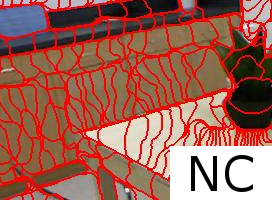
\includegraphics{pictures/nyu-test-1-nc-excerpt}
            }
            &
            \resizebox{\linewidth}{!}{
                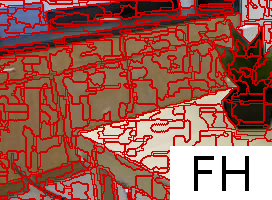
\includegraphics{pictures/nyu-test-1-fh-excerpt}
            }
            &
            \resizebox{\linewidth}{!}{
                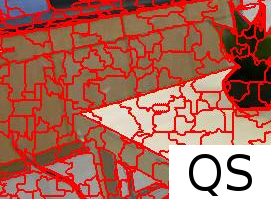
\includegraphics{pictures/nyu-test-1-qs-excerpt}
            }
            &
            \resizebox{\linewidth}{!}{
                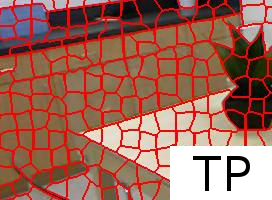
\includegraphics{pictures/nyu-test-1-tp-excerpt}
            }
            &
            \resizebox{\linewidth}{!}{
                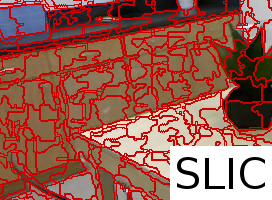
\includegraphics{pictures/nyu-test-1-orislic-excerpt}
            }
            &
            \resizebox{\linewidth}{!}{
                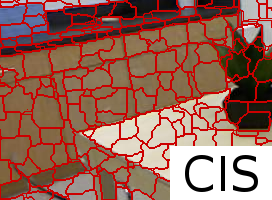
\includegraphics{pictures/nyu-test-1-cis-excerpt}
            }
            &
            \resizebox{\linewidth}{!}{
                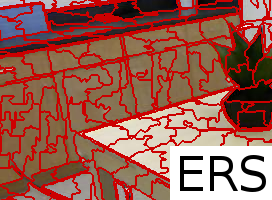
\includegraphics{pictures/nyu-test-1-ers-excerpt}
            }
            \\
            \resizebox{\linewidth}{!}{
                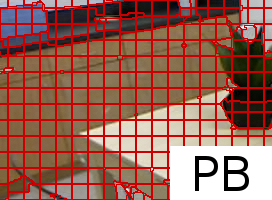
\includegraphics{pictures/nyu-test-1-pb-excerpt}
            }
            &
            \resizebox{\linewidth}{!}{
                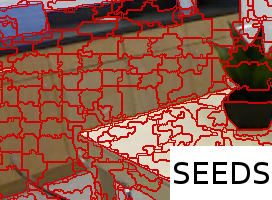
\includegraphics{pictures/nyu-test-1-oriseedsmp-excerpt}
            }
            &
            \resizebox{\linewidth}{!}{
                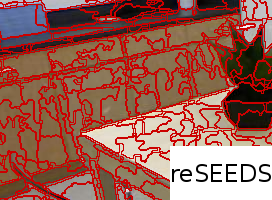
\includegraphics{pictures/nyu-test-1-reseedsmp-excerpt}
            }
            &
            \resizebox{\linewidth}{!}{
                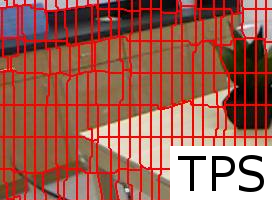
\includegraphics{pictures/nyu-test-1-tps-excerpt}
            }
            &
            \resizebox{\linewidth}{!}{
                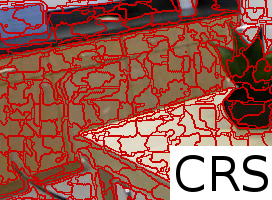
\includegraphics{pictures/nyu-test-1-crs-excerpt}
            }
            &
            \resizebox{\linewidth}{!}{
                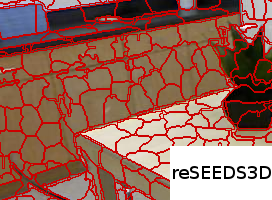
\includegraphics{pictures/nyu-test-1-seeds3d-excerpt}
            }
            &
            \resizebox{\linewidth}{!}{
                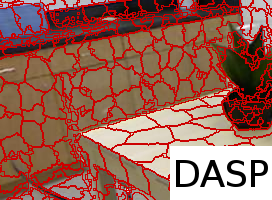
\includegraphics{pictures/nyu-test-1-dasp-beta-0-05-excerpt}
            }
            &
            \resizebox{\linewidth}{!}{
                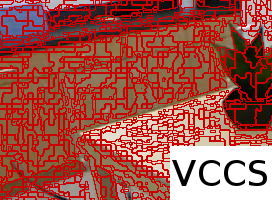
\includegraphics{pictures/nyu-test-1-vccs-excerpt}
            }            
        \end{tabularx}
        \vspace{-2.5mm}
        \caption{Superpixel segmentations obtained for an example image from the NYUV2. From left to right, top to bottom: original image, \textit{NC}, \textit{FH}, \textit{QS}, \textit{TP}, \textit{SLIC}, \textit{CIS}, \textit{ERS}, \textit{PB}, \textit{SEEDS}, \textit{reSEEDS}, \textit{TPS}, \textit{CRS}, \textit{reSEEDS3D}, \textit{DASP}, \textit{VCCS}. Note that \textit{reSEEDS3D}, \textit{DASP} and \textit{VCCS} use depth information for superpixel segmentation. Approximately $840$ superpixels have been computed for the whole image.}
        \label{fig:qualitative-nyu}
    \end{figure}
    
    Both \textit{FH} and \textit{QS} produce highly irregular superpixels. However, they are able to capture small details and all important boundaries. Furthermore, note that \textit{QS} produces more superpixels in highly textured areas. In contrast, \textit{TP} generates highly compact superpixels at the expense of missing several boundaries. \textit{CRS} and \textit{ERS} produce irregular superpixels with good boundary adherence and are more visually appealing than superpixels generated by \textit{FH} or \textit{QS}. While \textit{PB} shows reasonable results on the BSDS500, producing irregular and small superpixels, results on the NYUV2 appear to be unfinished and of poor quality. Similarly, \textit{TPS} produces unfinished superpixel segmentations on both datasets. Both \textit{SLIC} and \textit{CRS} provide a compactness parameter which has been traded off for boundary adherence during parameter optimization. Thus, the generated superpixels are irregular and not compact, especially on the NYUV2. The original implementation of \textit{SEEDS} produces highly irregular superpixels capturing the majority of boundaries. Our implementation, \textit{reSEEDS}, shows similar behavior.
    % {\color{red} However, due to an additional compactness parameter discussed in \cite{VanDenBerghBoixRoigVanGool:2013}, produces more regular superpixels in uniformly colored regions.}
    
    \begin{figure}[t]
	\centering
	\begin{tabularx}{\linewidth}{@{}Y@{}Y@{} | Y@{}Y@{}Y@{}}
        \resizebox{0.98\linewidth}{!}{
		    \begin{tikzpicture}
			    \begin{axis}[
					    height=6.4cm,
					    width=3cm,
					    y label style={at={(axis description cs:0.15,1.01)},anchor=south,rotate=-90},
					    xlabel=Superpixels,
					    ylabel=$Rec$,
					    ymin=0.9,
					    ymax=1,
					    xmin=100,
					    xmax=1200,
					    xtick={400,1000},
					    cycle list name=comparison bsd]
					
				    % NC
				    \addplot+[thick] table [row sep=newline,trim cells=true,x=K,y=Rec] {data/nc-bsd.csv};
				    \label{plot:evaluation-comparison-nc-rec-bsd}
				
				    % FH
				    \addplot+[thick] table [row sep=newline,trim cells=true,x=K,y=Rec] {data/fh-bsd-test.csv};
				    \label{plot:evaluation-comparison-fh-rec-bsd}
				
				    % QS
				    \addplot+[thick] table [row sep=newline,trim cells=true,x=K,y=Rec] {data/qs-bsd-test.csv};
				    \label{plot:evaluation-comparison-qs-rec-bsd}
				
				    % TP
				    \addplot+[thick] table [row sep=newline,trim cells=true,x=K,y=Rec] {data/tp-bsd-test.csv};
				    \label{plot:evaluation-comparison-tp-rec-bsd}
				
				    % oriSLIC
				    \addplot+[thick] table [row sep=newline,trim cells=true,x=K,y=Rec] {data/orislic-bsd-test.csv};
				    \label{plot:evaluation-comparison-orislic-rec-bsd}
				
				    % CIS
				    \addplot+[thick] table [row sep=newline,trim cells=true,x=K,y=Rec] {data/cis-bsd-test.csv};
				    \label{plot:evaluation-comparison-cis-rec-bsd}
				
				    % ERS
				    \addplot+[thick] table [row sep=newline,trim cells=true,x=K,y=Rec] {data/ers-bsd-test.csv};
				    \label{plot:evaluation-comparison-ers-rec-bsd}
				
				    % PB
				    \addplot+[thick] table [row sep=newline,trim cells=true,x=K,y=Rec] {data/pb-bsd-test.csv};
				    \label{plot:evaluation-comparison-pb-rec-bsd}
				
				    % SEEDSmp
				    \addplot+[thick] table [row sep=newline,trim cells=true,x=K,y=Rec] {data/oriseedsmp-bsd-test.csv};
				    \label{plot:evaluation-comparison-oriseedsmp-rec-bsd}
				
                    % reSEEDSmp
				    \addplot+[thick] table [row sep=newline,trim cells=true,x=K,y=Rec] {data/reseedsmp-bsd-test.csv};
				    \label{plot:evaluation-comparison-reseedssm-rec-bsd}

				    % reSEEDSmp*
				    %\addplot+[thick] table [row sep=newline,trim cells=true,x=K,y=Rec] {data/reseedssm-bsd-test.csv};
				    %\label{plot:evaluation-comparison-reseedssm-rec-bsd}
				
				    % TPS
				    \addplot+[thick] table [row sep=newline,trim cells=true,x=K,y=Rec] {data/tps-bsd-test.csv};
				    \label{plot:evaluation-comparison-tps-rec-bsd}
				
				    % CRS
				    \addplot+[thick] table [row sep=newline,trim cells=true,x=K,y=Rec] {data/crs-bsd-test.csv};
				    \label{plot:evaluation-comparison-crs-rec-bsd}
			    \end{axis}
		    \end{tikzpicture}
		}
	    &
	    \resizebox{0.98\linewidth}{!}{
		    \begin{tikzpicture}
			    \begin{axis}[
					    height=6.4cm,
					    width=3cm,
					    y label style={at={(axis description cs:0.15,1.01)},anchor=south,rotate=-90},
					    xlabel=Superpixels,
					    ylabel=$UE$,
					    ymin=0.025,
					    ymax=0.1,
					    xmin=100,
					    xmax=1200,
					    xtick={400,1000},
					    cycle list name=comparison bsd]
				
				    % NC
				    \addplot+[thick] table [row sep=newline,trim cells=true,x=K,y=UE] {data/nc-bsd.csv};
				    \label{plot:evaluation-comparison-nc-ue-bsd}
				
				    % FH
				    \addplot+[thick] table [row sep=newline,trim cells=true,x=K,y=UE] {data/fh-bsd-test.csv};
				    \label{plot:evaluation-comparison-fh-ue-bsd}
				
				    % QS
				    \addplot+[thick] table [row sep=newline,trim cells=true,x=K,y=UE] {data/qs-bsd-test.csv};
				    \label{plot:evaluation-comparison-qs-ue-bsd}
				
				    % TP
				    \addplot+[thick] table [row sep=newline,trim cells=true,x=K,y=UE] {data/tp-bsd-test.csv};
				    \label{plot:evaluation-comparison-tp-ue-bsd}
				
				    % oriSLIC
				    \addplot+[thick] table [row sep=newline,trim cells=true,x=K,y=UE] {data/orislic-bsd-test.csv};
				    \label{plot:evaluation-comparison-orislic-ue-bsd}
				
				    % CIS
				    \addplot+[thick] table [row sep=newline,trim cells=true,x=K,y=UE] {data/cis-bsd-test.csv};
				    \label{plot:evaluation-comparison-cis-ue-bsd}
				
				    % ERS
				    \addplot+[thick] table [row sep=newline,trim cells=true,x=K,y=UE] {data/ers-bsd-test.csv};
				    \label{plot:evaluation-comparison-ers-ue-bsd}
				
				    % PB
				    \addplot+[thick] table [row sep=newline,trim cells=true,x=K,y=UE] {data/pb-bsd-test.csv};
				    \label{plot:evaluation-comparison-pb-ue-bsd}
				
				    % SEEDSmp
				    \addplot+[thick] table [row sep=newline,trim cells=true,x=K,y=UE] {data/oriseedsmp-bsd-test.csv};
				    \label{plot:evaluation-comparison-oriseedsmp-ue-bsd}
				
				    % reSEEDSmp
				    \addplot+[thick] table [row sep=newline,trim cells=true,x=K,y=UE] {data/reseedsmp-bsd-test.csv};
				    \label{plot:evaluation-comparison-reseedssm-ue-bsd}
				
                    % reSEEDSmp*
				    %\addplot+[thick] table [row sep=newline,trim cells=true,x=K,y=UE] {data/reseedssm-bsd-test.csv};
				    %\label{plot:evaluation-comparison-reseedssm-ue-bsd}

				    % TPS
				    \addplot+[thick] table [row sep=newline,trim cells=true,x=K,y=UE] {data/tps-bsd-test.csv};
				    \label{plot:evaluation-comparison-tps-ue-bsd}
				
				    % CRS
				    \addplot+[thick] table [row sep=newline,trim cells=true,x=K,y=UE] {data/crs-bsd-test.csv};
				    \label{plot:evaluation-comparison-crs-ue-bsd}
			    \end{axis}
			    %\matrix[%
			    %		matrix of nodes,%
			    %		anchor=north west,%
			    %		inner sep=0.15em,%
			    %		nodes={font=\scriptsize},%
			    %		column 1/.append style={anchor=base west},%
			    %	] at ($(current axis.north east) + (0.25,0)$) {
			    %		BSDS500:\\
			    %		\ref{plot:evaluation-comparison-nc-ue-bsd} \textit{NC}
			    %		\ref{plot:evaluation-comparison-fh-ue-bsd} \textit{FH}\\
			    %		\ref{plot:evaluation-comparison-qs-ue-bsd} \textit{QS}
			    %		\ref{plot:evaluation-comparison-tp-ue-bsd} \textit{TP}\\
			    %		\ref{plot:evaluation-comparison-orislic-ue-bsd} \textit{oriSLIC}\\
			    %		% vlSLIC
			    %		\ref{plot:evaluation-comparison-cis-ue-bsd} \textit{CIS}
			    %		\ref{plot:evaluation-comparison-ers-ue-bsd} \textit{ERS}\\
			    %		\ref{plot:evaluation-comparison-pb-ue-bsd} \textit{PB}
			    %		\ref{plot:evaluation-comparison-crs-ue-bsd} \textit{CRS}\\
			    %		\ref{plot:evaluation-comparison-oriseedsmp-ue-bsd} \textit{SEEDSmp}\\
			    %		\ref{plot:evaluation-comparison-reseedssm-ue-bsd} \textit{reSEEDSmp*}\\
			    %		\ref{plot:evaluation-comparison-tps-ue-bsd} \textit{TPS}\\
			    %	};
		    \end{tikzpicture}
		}
	    &
	    \resizebox{\linewidth}{!}{
		    \begin{tikzpicture}
			    \begin{axis}[
					    height=6.4cm,
					    width=3cm,
					    y label style={at={(axis description cs:0.15,1.01)},anchor=south,rotate=-90},
					    xlabel=Superpixels,
					    ylabel=$Rec$,
					    ymin=0.9,
					    ymax=1,
					    xmin=300,
					    xmax=1700,
					    xtick={500,1500},
					    cycle list name=comparison nyu]
				
				    % NC
				    \addplot+[thick] table [row sep=newline,trim cells=true,x=K,y=Rec] {data/nc-nyu.csv};
				    \label{plot:evaluation-comparison-nc-rec-nyu}
				
				    % FH
				    \addplot+[thick] table [row sep=newline,trim cells=true,x=K,y=Rec] {data/fh-nyu-test.csv};
				    \label{plot:evaluation-comparison-fh-rec-nyu}
				
				    % QS
				    \addplot+[thick] table [row sep=newline,trim cells=true,x=K,y=Rec] {data/qs-nyu-test.csv};
				    \label{plot:evaluation-comparison-qs-rec-nyu}
				
				    % TP
				    \addplot+[thick] table [row sep=newline,trim cells=true,x=K,y=Rec] {data/tp-nyu-test.csv};
				    \label{plot:evaluation-comparison-tp-rec-nyu}
				
				    % oriSLIC
				    \addplot+[thick] table [row sep=newline,trim cells=true,x=K,y=Rec] {data/orislic-nyu-test.csv};
				    \label{plot:evaluation-comparison-orislic-rec-nyu}
				
				    % SLIC3D
				    %\addplot+[thick] table [row sep=newline,trim cells=true,x=K,y=Rec] {data/slic3d-nyu-test.csv};
				    %\label{plot:evaluation-comparison-slic3d-rec-nyu}
				
				    % CIS
				    \addplot+[thick] table [row sep=newline,trim cells=true,x=K,y=Rec] {data/cis-nyu-test.csv};
				    \label{plot:evaluation-comparison-cis-rec-nyu}
				
				    % ERS
				    \addplot+[thick] table [row sep=newline,trim cells=true,x=K,y=Rec] {data/ers-nyu-test.csv};
				    \label{plot:evaluation-comparison-ers-rec-nyu}
				
				    % PB
				    \addplot+[thick] table [row sep=newline,trim cells=true,x=K,y=Rec] {data/pb-nyu-test.csv};
				    \label{plot:evaluation-comparison-pb-rec-nyu}
				
				    % SEEDSmp
				    \addplot+[thick] table [row sep=newline,trim cells=true,x=K,y=Rec] {data/oriseedsmp-nyu-test.csv};
				    \label{plot:evaluation-comparison-oriseedsmp-rec-nyu}
				
                    % reSEEDSmp
				    \addplot+[thick] table [row sep=newline,trim cells=true,x=K,y=Rec] {data/reseedsmp-nyu-test.csv};
				    \label{plot:evaluation-comparison-reseedssm-rec-nyu}

				    % reSEEDSmp*
				    %\addplot+[thick] table [row sep=newline,trim cells=true,x=K,y=Rec] {data/reseedssm-nyu-test.csv};
				    %\label{plot:evaluation-comparison-reseedssm-rec-nyu}
				
				    % reSEEDS3D
				    \addplot+[thick] table [row sep=newline,trim cells=true,x=K,y=Rec] {data/seeds3d-nyu-test.csv};
				    \label{plot:evaluation-comparison-seeds3d-rec-nyu}
				
				    % DASP
				    \addplot+[thick] table [row sep=newline,trim cells=true,x=K,y=Rec] {data/dasp-nyu-test.csv};
				    \label{plot:evaluation-comparison-dasp-rec-nyu}
				
				    % TPS
				    \addplot+[thick] table [row sep=newline,trim cells=true,x=K,y=Rec] {data/tps-nyu-test.csv};
				    \label{plot:evaluation-comparison-tps-rec-nyu}
				
				    % CRS
				    \addplot+[thick] table [row sep=newline,trim cells=true,x=K,y=Rec] {data/crs-nyu-test.csv};
				    \label{plot:evaluation-comparison-crs-rec-nyu}
				
				    % DCRS
				
				    % VCCS
				    \addplot+[thick] table [row sep=newline,trim cells=true,x=K,y=Rec] {data/vccs-depth-test.csv};
				    \label{plot:evaluation-comparison-vccs-rec-nyu}
			    \end{axis}
		    \end{tikzpicture}
		}
	    &
	    \resizebox{\linewidth}{!}{
		    \begin{tikzpicture}
			    \begin{axis}[
					    height=6.4cm,
					    width=3cm,
					    y label style={at={(axis description cs:0.15,1.01)},anchor=south,rotate=-90},
					    xlabel=Superpixels,
					    ylabel=$UE$,
					    ymin=0.07,
					    ymax=0.17,
					    xmin=300,
					    xmax=1700,
					    xtick={500,1500},
					    cycle list name=comparison nyu]
				
				    % NC
				    \addplot+[thick] table [row sep=newline,trim cells=true,x=K,y=UE] {data/nc-nyu.csv};
				    \label{plot:evaluation-comparison-nc-ue-nyu}
				
				    % FH
				    \addplot+[thick] table [row sep=newline,trim cells=true,x=K,y=UE] {data/fh-nyu-test.csv};
				    \label{plot:evaluation-comparison-fh-ue-nyu}
				
				    % QS
				    \addplot+[thick] table [row sep=newline,trim cells=true,x=K,y=UE] {data/qs-nyu-test.csv};
				    \label{plot:evaluation-comparison-qs-ue-nyu}
				
				    % TP
				    \addplot+[thick] table [row sep=newline,trim cells=true,x=K,y=UE] {data/tp-nyu-test.csv};
				    \label{plot:evaluation-comparison-tp-ue-nyu}
				
				    % oriSLIC
				    \addplot+[thick] table [row sep=newline,trim cells=true,x=K,y=UE] {data/orislic-nyu-test.csv};
				    \label{plot:evaluation-comparison-orislic-ue-nyu}
				
				    % SLIC3D
				    %\addplot+[thick] table [row sep=newline,trim cells=true,x=K,y=UE] {data/slic3d-nyu-test.csv};
				    %\label{plot:evaluation-comparison-slic3d-ue-nyu}
				
				    % CIS
				    \addplot+[thick] table [row sep=newline,trim cells=true,x=K,y=UE] {data/cis-nyu-test.csv};
				    \label{plot:evaluation-comparison-cis-ue-nyu}
				
				    % ERS
				    \addplot+[thick] table [row sep=newline,trim cells=true,x=K,y=UE] {data/ers-nyu-test.csv};
				    \label{plot:evaluation-comparison-ers-ue-nyu}
				
				    % PB
				    \addplot+[thick] table [row sep=newline,trim cells=true,x=K,y=UE] {data/pb-nyu-test.csv};
				    \label{plot:evaluation-comparison-pb-ue-nyu}
				
				    % SEEDSmp
				    \addplot+[thick] table [row sep=newline,trim cells=true,x=K,y=UE] {data/oriseedsmp-nyu-test.csv};
				    \label{plot:evaluation-comparison-oriseedsmp-ue-nyu}
				
				    % reSEEDSmp
				    \addplot+[thick] table [row sep=newline,trim cells=true,x=K,y=UE] {data/reseedsmp-nyu-test.csv};
				    \label{plot:evaluation-comparison-reseedssm-ue-nyu}
				
				    % reSEEDSmp*
				    %\addplot+[thick] table [row sep=newline,trim cells=true,x=K,y=UE] {data/reseedssm-nyu-test.csv};
				    %\label{plot:evaluation-comparison-reseedssm-ue-nyu}
				
				    % reSEEDS3D
				    \addplot+[thick] table [row sep=newline,trim cells=true,x=K,y=UE] {data/seeds3d-nyu-test.csv};
				    \label{plot:evaluation-comparison-seeds3d-ue-nyu}
				
				    % DASP
				    \addplot+[thick] table [row sep=newline,trim cells=true,x=K,y=UE] {data/dasp-nyu-test.csv};
				    \label{plot:evaluation-comparison-dasp-ue-nyu}
				
				    % TPS
				    \addplot+[thick] table [row sep=newline,trim cells=true,x=K,y=UE] {data/tps-nyu-test.csv};
				    \label{plot:evaluation-comparison-tps-ue-nyu}
				
				    % CRS
				    \addplot+[thick] table [row sep=newline,trim cells=true,x=K,y=UE] {data/crs-nyu-test.csv};
				    \label{plot:evaluation-comparison-crs-ue-nyu}
				
				    % DCRS
				
				    % VCCS
				    \addplot+[thick] table [row sep=newline,trim cells=true,x=K,y=UE] {data/vccs-depth-test.csv};
				    \label{plot:evaluation-comparison-vccs-ue-nyu}
			    \end{axis}
		    \end{tikzpicture}
		}
	    &
	    \resizebox{\linewidth}{!}{
	        \begin{tikzpicture}
			    \matrix[%
					    matrix of nodes,%
					    anchor=north west,%
					    inner sep=0.11em,%
					    nodes={font=\scriptsize},%
					    column 1/.append style={anchor=base west},%
				    ] at ($(current axis.north east) - (0.25,0)$) {
					    \ref{plot:evaluation-comparison-nc-ue-nyu} \textit{NC}\\
					    \ref{plot:evaluation-comparison-fh-ue-nyu} \textit{FH}\\
					    \ref{plot:evaluation-comparison-qs-ue-nyu} \textit{QS}\\
					    \ref{plot:evaluation-comparison-tp-ue-nyu} \textit{TP}\\
					    \ref{plot:evaluation-comparison-orislic-ue-nyu} \textit{SLIC}\\
					    %\ref{plot:evaluation-comparison-slic3d-ue-nyu} \textit{SLIC3D}\\
					    % SLIC3D
					    \ref{plot:evaluation-comparison-cis-ue-nyu} \textit{CIS}\\
					    \ref{plot:evaluation-comparison-ers-ue-nyu} \textit{ERS}\\
					    \ref{plot:evaluation-comparison-pb-ue-nyu} \textit{PB}\\
					    \ref{plot:evaluation-comparison-crs-ue-nyu} \textit{CRS}\\
					    \ref{plot:evaluation-comparison-oriseedsmp-ue-nyu} \textit{SEEDS}\\
					    \ref{plot:evaluation-comparison-reseedssm-ue-nyu} \textit{reSEEDS}\\
					    \ref{plot:evaluation-comparison-seeds3d-ue-nyu} \textit{reSEEDS3D}\\
					    \ref{plot:evaluation-comparison-dasp-ue-nyu} \textit{DASP}\\
					    \ref{plot:evaluation-comparison-tps-ue-nyu} \textit{TPS}\\
					    % DCRS
					    \ref{plot:evaluation-comparison-vccs-ue-nyu} \textit{VCCS}\\
					    \phantom{a}\\
					    \phantom{a}\\
					    \phantom{a}\\
					    \phantom{a}\\
					    \phantom{a}\\
					    \phantom{a}\\
					    \phantom{a}\\
					    \phantom{a}\\
					    \phantom{a}\\
					    \phantom{a}\\
				    };
		    \end{tikzpicture}
		}
	\end{tabularx}
	\vspace{-3mm}
	\caption{Comparison of thirteen superpixel algorithms with respect to Boundary Recall ($Rec$) and Undersegmentation Error ($UE$) on the test sets of the BSDS500 (left) and the NYUV2 (right).
	Note that for visualization purposes only a small part of the range of both metrics is shown.
	}
	\label{fig:quantitative}
\end{figure}
    
    Intuitively, depth information allows to adapt superpixels to the underlying three-dimensional structure. While \textit{DASP} is able to resemble this structure at least in parts, \textit{VCCS} produces highly irregular superpixels. This may be due to the fact that \textit{DASP} adapts the number of superpixels according to depth, whereas \textit{VCCS} directly operates within the point cloud and merely the back projection is shown. As result, the generated superpixels occur irregular and voxelization (see \cite{PaponAbramovSchoelerWoergoetter:2013}) is still visible.
    % In particular, the process of voxelization is still visible.
    % Except for some artifacts, \textit{reSEEDS3D} produces slightly more compact superpixels compared to the other approaches using depth information. 
    Compared to \textit{DASP}, \textit{reSEEDS3D} generates slightly less irregular superpixels with better boundary adherence.
    
    \vspace{-1.5mm}
    \subsection{Quantitative}
    \label{subsec:quantitative}
    \vspace{-0.5mm}
    
    % Quantitative evaluation is guided by Boundary Recall and Undersegmentation, shown in Figure \ref{fig:quantitative} with respect to the number of superpixels, as well as runtime, shown in Figure \ref{fig:runtime}.

    % The quantiative comparison shows Boundary Recall and Undersegmentation Error as a function of the number of superpixels. Achieving high Boundary Recall and low Undersegmentation Error while generating few superpixels is an indicator of superior performance.
    
    % TODO: averaged over the test sets.
    The quantitative comparison is based on Boundary Recall and Undersegmentation Error, averaged over the test sets, as a function of the number of superpixels. As shown in Figure \ref{fig:quantitative}, \textit{FH} performs excellent on both datasets and is only outperformed by \textit{VCCS}. However, as \textit{VCCS} operates within point clouds, these results are hardly comparable. In addition, \textit{FH} is closely followed by approaches such as \textit{QS}, \textit{SLIC}, \textit{CRS} and \textit{ERS}. Our implementation of \textit{SEEDS}, \textit{reSEEDS}, is able to keep up with \textit{FH}, while consistently outperforming the original implementation. Unfortunately, as shown by \textit{reSEEDS3D}, depth information may not necessarily improve performance. This is supported by the poor performance of \textit{DASP}. In addition, our implementation of \textit{SEEDS} demonstrates that any ranking extracted from Figure \ref{fig:quantitative} is possibly challenged by revising existing implementations. This also justifies a qualitative comparison as performed in Section~\ref{subsec:qualitative}.

    \begin{figure}[t]
	\centering
	\begin{tabularx}{\linewidth}{@{}Y@{}Y@{}Y@{}Y@{}}
	    \resizebox{\linewidth}{!}{
		    \begin{tikzpicture}
			    \begin{axis}[
					    height=4.3cm,
					    width=3.25cm,
					    y label style={at={(axis description cs:0.15,1.01)},anchor=south,rotate=-90},
					    xlabel=Superpixels,
					    ylabel=$Rec$,
					    ymin=0.9,
					    ymax=1,
					    xmin=300,
					    xmax=1700,
					    xtick={500,1500},
					    cycle list name=runtime nyu]
				
				    % FH
				    \addplot+[thick] table [row sep=newline,trim cells=true,x=K,y=Rec] {data/fh-nyu-test.csv};
				    \label{plot:evaluation-comparison-iteration-fh-rec-nyu}
				
				    % oriSLIC 1it
				    \addplot+[thick] table [row sep=newline,trim cells=true,x=K,y=Rec] {data/orislic1it-nyu-test.csv};
				    \label{plot:evaluation-comparison-iteration-orislic1it-rec-nyu}
				    
				    % oriSLIC
				    \addplot+[thick] table [row sep=newline,trim cells=true,x=K,y=Rec] {data/orislic-nyu-test.csv};
				    \label{plot:evaluation-comparison-orislic-rec-nyu}
				    
				    % SEEDSmp 1it
				    \addplot+[thick] table [row sep=newline,trim cells=true,x=K,y=Rec] {data/oriseedsmp1it-nyu-test.csv};
				    \label{plot:evaluation-comparison-iteration-oriseedsmp1it-rec-nyu}
				
				    % SEEDSmp
				    \addplot+[thick] table [row sep=newline,trim cells=true,x=K,y=Rec] {data/oriseedsmp-nyu-test.csv};
				    \label{plot:evaluation-comparison-iteration-oriseedsmp-rec-nyu}
				
				    % reSEEDSmp
				    %\addplot+[thick] table [row sep=newline,trim cells=true,x=K,y=Rec] {data/reseedsmp1it-nyu-test.csv};
				    %\label{plot:evaluation-comparison-iteration-reseedsmp-rec-nyu}
				
				    % reSEEDSmp 1it
				    \addplot+[thick] table [row sep=newline,trim cells=true,x=K,y=Rec] {data/reseedsmp1it-nyu-test.csv};
				    \label{plot:evaluation-comparison-iteration-reseedssm1it-rec-nyu}
				
				    % reSEEDSmp* 1it
				    %\addplot+[thick] table [row sep=newline,trim cells=true,x=K,y=Rec] {data/reseedssm1it-nyu-test.csv};
				    %\label{plot:evaluation-comparison-iteration-reseedssm1it-rec-nyu}
				
				    % reSEEDSmp
				    \addplot+[thick] table [row sep=newline,trim cells=true,x=K,y=Rec] {data/reseedsmp-nyu-test.csv};
				    \label{plot:evaluation-comparison-iteration-reseedssm-rec-nyu}
				
				    % reSEEDSmp*
				    %\addplot+[thick] table [row sep=newline,trim cells=true,x=K,y=Rec] {data/reseedssm-nyu-test.csv};
				    %\label{plot:evaluation-comparison-iteration-reseedssm-rec-nyu}
				
				    % reSEEDS3D
				    \addplot+[thick] table [row sep=newline,trim cells=true,x=K,y=Rec] {data/seeds3d1it-nyu-test.csv};
				    \label{plot:evaluation-comparison-iteration-seeds3d-rec-nyu}
				
				    % DASP
				    \addplot+[thick] table [row sep=newline,trim cells=true,x=K,y=Rec] {data/dasp-nyu-test.csv};
				    \label{plot:evaluation-comparison-iteration-dasp-rec-nyu}
				
				    % VCCS
				    \addplot+[thick] table [row sep=newline,trim cells=true,x=K,y=Rec] {data/vccs-depth-test.csv};
				    \label{plot:evaluation-comparison-iteration-vccs-rec-nyu}
				
			    \end{axis}
		    \end{tikzpicture}
		}
		&
		\resizebox{\linewidth}{!}{
		    \begin{tikzpicture}
			    \begin{axis}[
					    height=4.3cm,
					    width=3.25cm,
					    y label style={at={(axis description cs:0.15,1.01)},anchor=south,rotate=-90},
					    xlabel=Superpixels,
					    ylabel=$UE$,
					    ymin=0.07,
					    ymax=0.17,
					    xmin=300,
					    xmax=1700,
					    xtick={500,1500},
					    cycle list name=runtime nyu]
				
				    % FH
				    \addplot+[thick] table [row sep=newline,trim cells=true,x=K,y=UE] {data/fh-nyu-test.csv};
				    \label{plot:evaluation-comparison-iteration-fh-ue-nyu}
				
				    % oriSLIC 1it
				    \addplot+[thick] table [row sep=newline,trim cells=true,x=K,y=UE] {data/orislic1it-nyu-test.csv};
				    \label{plot:evaluation-comparison-iteration-orislic1it-ue-nyu}
				
				    % oriSLIC
				    \addplot+[thick] table [row sep=newline,trim cells=true,x=K,y=UE] {data/orislic-nyu-test.csv};
				    \label{plot:evaluation-comparison-iteration-orislic-ue-nyu}
				
				    % SLIC3D
				    %\addplot+[thick] table [row sep=newline,trim cells=true,x=K,y=UE] {data/slic3d-nyu-test.csv};
				    %\label{plot:evaluation-comparison-slic3d-ue-nyu}
				
				    % SEEDSmp 1it
				    \addplot+[thick] table [row sep=newline,trim cells=true,x=K,y=UE] {data/oriseedsmp1it-nyu-test.csv};
				    \label{plot:evaluation-comparison-iteration-oriseedsmp1it-ue-nyu}
				
				    % SEEDSmp
				    \addplot+[thick] table [row sep=newline,trim cells=true,x=K,y=UE] {data/oriseedsmp-nyu-test.csv};
				    \label{plot:evaluation-comparison-iteration-oriseedsmp-ue-nyu}
				
				    % reSEEDSmp
				    %\addplot+[thick] table [row sep=newline,trim cells=true,x=K,y=UE] {data/reseedsmp1it-nyu-test.csv};
				    %\label{plot:evaluation-comparison-iteration-reseedsmp-ue-nyu}
				
				    % reSEEDSmp 1it
				    \addplot+[thick] table [row sep=newline,trim cells=true,x=K,y=UE] {data/reseedsmp1it-nyu-test.csv};
				    \label{plot:evaluation-comparison-iteration-reseedssm1it-ue-nyu}
				
				    % reSEEDSmp* 1it
				    %\addplot+[thick] table [row sep=newline,trim cells=true,x=K,y=UE] {data/reseedssm1it-nyu-test.csv};
				    %\label{plot:evaluation-comparison-iteration-reseedssm1it-ue-nyu}
				
				    % reSEEDSmp
				    \addplot+[thick] table [row sep=newline,trim cells=true,x=K,y=UE] {data/reseedsmp-nyu-test.csv};
				    \label{plot:evaluation-comparison-iteration-reseedssm-ue-nyu}
				
				    % reSEEDSmp*
				    %\addplot+[thick] table [row sep=newline,trim cells=true,x=K,y=UE] {data/reseedssm-nyu-test.csv};
				    %\label{plot:evaluation-comparison-iteration-reseedssm-ue-nyu}
				
				    % reSEEDS3D
				    \addplot+[thick] table [row sep=newline,trim cells=true,x=K,y=UE] {data/seeds3d1it-nyu-test.csv};
				    \label{plot:evaluation-comparison-iteration-seeds3d-ue-nyu}
				
				    % DASP
				    \addplot+[thick] table [row sep=newline,trim cells=true,x=K,y=UE] {data/dasp-nyu-test.csv};
				    \label{plot:evaluation-comparison-iteration-dasp-ue-nyu}
				
				    % VCCS
				    \addplot+[thick] table [row sep=newline,trim cells=true,x=K,y=UE] {data/vccs-depth-test.csv};
				    \label{plot:evaluation-comparison-iteration-vccs-ue-nyu}
				
			    \end{axis}
		    \end{tikzpicture}
	    }
	    &
	    \resizebox{\linewidth}{!}{
		    \begin{tikzpicture}
			    \begin{axis}[
					    height=4.1cm,
					    width=3.25cm,
					    y label style={at={(axis description cs:0.15,1.01)},anchor=south,rotate=-90},
					    xlabel=Superpixels,
					    ylabel=$t$,
					    ymin=0,
					    ymax=0.45,
					    xmin=300,
					    xmax=1700,
					    xtick={500,1500},
					    cycle list name=runtime nyu]
				
				    % FH
				    \addplot+[thick] table [row sep=newline,trim cells=true,x=K,y=t] {data/fh-nyu-test.csv};
				    \label{plot:evaluation-comparison-iteration-fh-t-nyu}
				
				    % oriSLIC 1it
				    \addplot+[thick] table [row sep=newline,trim cells=true,x=K,y=t] {data/orislic1it-nyu-test.csv};
				    \label{plot:evaluation-comparison-iteration-orislic1it-t-nyu}
				
				    % oriSLIC
				    \addplot+[thick] table [row sep=newline,trim cells=true,x=K,y=t] {data/orislic-nyu-test.csv};
				    \label{plot:evaluation-comparison-iteration-orislic-t-nyu}
				
				    % SEEDSmp 1it
				    \addplot+[thick] table [row sep=newline,trim cells=true,x=K,y=t] {data/oriseedsmp1it-nyu-test.csv};
				    \label{plot:evaluation-comparison-iteration-oriseedsmp1it-t-nyu}
				
				    % SEEDSmp
				    \addplot+[thick] table [row sep=newline,trim cells=true,x=K,y=t] {data/oriseedsmp-nyu-test.csv};
				    \label{plot:evaluation-comparison-iteration-oriseedsmp-t-nyu}
				
				    % reSEEDSmp 1it
				    \addplot+[thick] table [row sep=newline,trim cells=true,x=K,y=t] {data/reseedsmp1it-nyu-test.csv};
				    \label{plot:evaluation-comparison-iteration-reseedssm1it-t-nyu}
				
				    % reSEEDSmp* 1it
				    %\addplot+[thick] table [row sep=newline,trim cells=true,x=K,y=t] {data/reseedssm1it-nyu-test.csv};
				    %\label{plot:evaluation-comparison-iteration-reseedssm1it-t-nyu}
				
				    % reSEEDSmp
				    \addplot+[thick] table [row sep=newline,trim cells=true,x=K,y=t] {data/reseedsmp-nyu-test.csv};
				    \label{plot:evaluation-comparison-iteration-reseedssm-t-nyu}
				
				    % reSEEDSmp*
				    %\addplot+[thick] table [row sep=newline,trim cells=true,x=K,y=t] {data/reseedssm-nyu-test.csv};
				    %\label{plot:evaluation-comparison-iteration-reseedssm-t-nyu}
				
				    % reSEEDS3D
				    \addplot+[thick] table [row sep=newline,trim cells=true,x=K,y=t] {data/seeds3d-nyu-test.csv};
				    \label{plot:evaluation-comparison-iteration-seeds3d-t-nyu}
				
				    % DASP
				    \addplot+[thick] table [row sep=newline,trim cells=true,x=K,y=t] {data/dasp-nyu-test.csv};
				    \label{plot:evaluation-comparison-iteration-dasp-t-nyu}
				
				    % VCCS
				    \addplot+[thick] table [row sep=newline,trim cells=true,x=K,y=t] {data/vccs-depth-test.csv};
				    \label{plot:evaluation-comparison-iteration-vccs-t-nyu}
			    \end{axis}
		    \end{tikzpicture}
		}
		&
		\resizebox{0.925\linewidth}{!}{
		    \begin{tikzpicture}
		        \matrix[%
				        matrix of nodes,%
				        anchor=north west,%
				        inner sep=0.15em,%
				        nodes={font=\scriptsize},%
				        column 1/.append style={anchor=base west},%
			        ] at ($(current axis.north east) + (0.25,0)$) {
				        \ref{plot:evaluation-comparison-iteration-fh-t-nyu} \textit{FH}\\
				        \ref{plot:evaluation-comparison-iteration-orislic1it-t-nyu} \textit{SLIC} $\ast$\\
				        \ref{plot:evaluation-comparison-iteration-orislic-t-nyu} \textit{SLIC}\\
				        \ref{plot:evaluation-comparison-iteration-oriseedsmp1it-t-nyu} \textit{SEEDS} $\ast$\\
				        \ref{plot:evaluation-comparison-iteration-oriseedsmp-t-nyu} \textit{SEEDS}\\
				        \ref{plot:evaluation-comparison-iteration-reseedssm1it-t-nyu} \textit{reSEEDS} $\ast$\\
				        \ref{plot:evaluation-comparison-iteration-reseedssm-t-nyu} \textit{reSEEDS}\\
				        \ref{plot:evaluation-comparison-iteration-seeds3d-t-nyu} \textit{reSEEDS3D}\\
				        \ref{plot:evaluation-comparison-iteration-dasp-t-nyu} \textit{DASP}\\
				        \ref{plot:evaluation-comparison-iteration-vccs-t-nyu} \textit{VCCS}\\
				        \phantom{a}\\
				        \phantom{a}\\
				        \phantom{a}\\
				        \phantom{a}\\
				        \phantom{a}\\
			        };
		    \end{tikzpicture}
        }
	\end{tabularx}
	\vspace{-3mm}
	\caption{Comparison of the runtime $t$ in seconds of superpixel algorithms requiring less than $0.5s$ per image on the NYUV2. \textit{SLIC}, \textit{SEEDS} and \textit{reSEEDS} may be optimized with respect to runtime by decreasing the number of iterations. These optimized versions are indicated by an $\ast$.}
	\label{fig:runtime}
\end{figure}
    
    Another important aspect of superpixel algorithms is runtime (measured using a 64bit machine with Intel Core i7-3770@3.4GHz, 16GB RAM and without GPU acceleration or multi-threading). Iterative algorithms such as \textit{SLIC} and \textit{SEEDS} may be optimized with respect to runtime by decreasing the number of iterations. Figure \ref{fig:runtime} compares these optimized versions to algorithms requiring less than $0.5s$ on the NYUV2 (images of size $608 \times 448$). The optimized versions of \textit{SLIC}, \textit{SEEDS} and \textit{reSEEDS}, indicated by an $\ast$, show significantly reduced runtime while providing similar performance in terms of Boundary Recall and Undersegmentation Error. The drop in performance is lowest for \textit{reSEEDS} -- Boundary Recall even increases -- which simultaneously shows the lowest runtime with $\sim0.05s$ per image. We also observe low runtimes for \textit{FH} and \textit{DASP}.
    
    \vspace{-1mm}
    \section{Conclusion}
    \vspace{-0.5mm}
    \label{sec:conclusion}

    Several algorithms provide both excellent performance and low runtime. Furthermore, including additional information such as depth may not necessarily improve performance. Therefore, additional criteria are necessary to asses superpixel algorithms. In particular, we find that visual quality, runtime and the provided parameters are among these criteria. Clearly, visual appearance is difficult to measure appropriately, however, it may have serious impact on possible applications. Furthermore, low runtime is desirable when using superpixel algorithms as pre-processing step, especially in real-time settings. Finally, parameters should be interpretable and easy to tune and algorithms providing a compactness parameter are preferable. In addition, as the number of superpixels can be understood as a lower bound on performance, we prefer algorithms offering direct control over the number of superpixels.
    
    In conclusion, while many algorithms provide excellent performance with respect to Undersegmentation Error \cite{LevinshteinStereKutulakosFleetDickinsonSiddiqi:2009,NeubertProtzel:2012} and Boundary Recall \cite{MartinFowlkesMalik:2004}, they lack control over the number of superpixels or a compactness parameter.
    % Further, the quantitative performance of many algorithms is not reflected in the qualitative assessment.
    % Further, for several algorithms, the quantitative performance does not necessarily reflect the perceived visual quality of the generated superpixel segmentations.
    Furthermore, these impressive results with respect to Boundary Recall and Undersegmentation Error do not necessarily reflect the perceived visual quality of the generated superpixel segmentations.
    
	\bibliographystyle{splncs03}
	\bibliography{paper}

\end{document}

